%!TEX root = ../../main.tex
\chapter{ユーザースキルの推薦機構}
本章ではユーザースキル推薦機構について述べる.

\section{スキルタグ}
スキルタグの実例を\ref{img:skill_tag}に示す.
システムの実装というタスクに対してRuby・JavaScript・LODのタグ,Tex構築というタスクに対してTexのタグが付与されている.

\begin{figure}[t]
	\begin{center}
		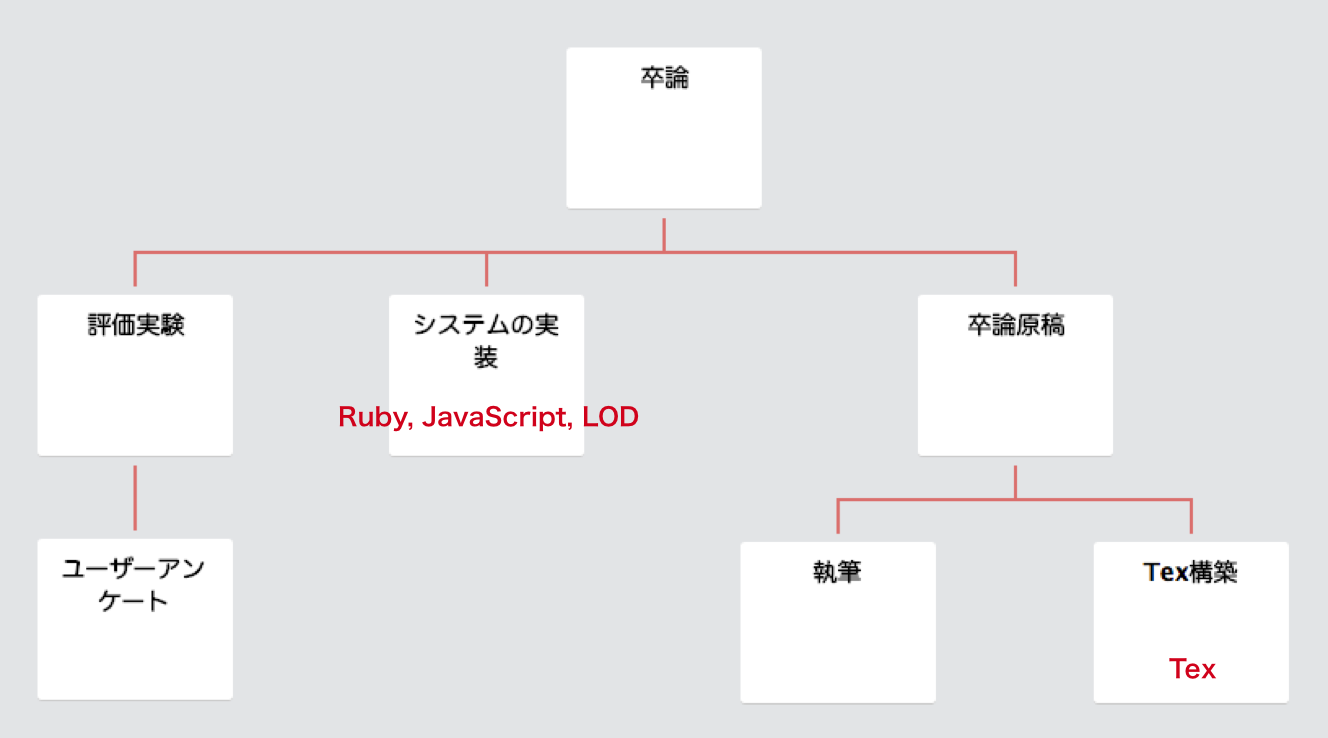
\includegraphics[width=0.9\linewidth]{assets/img/skill_tag.png}
		\caption{スキルタグ実例}
		\label{img:skill_tag}
	\end{center}
\end{figure}

\subsection{活用事例}
世界最大級のビジネス特化型ソーシャル・ネットワーキング・サービスであるLinkedIn\footnote{https://www.linkedin.com}や,
IT/Web業界最大級のソーシャル・リクルーティング・ツールであるWantedly\footnote{https://www.wantedly.com}や,
では,自分のスキルタグを登録することができる.
このスキルタグを用いて,ユーザー同士のマッチングをしたり,採用活動に活用している.

\section{ユーザースキルの推定}
本システムでは,そのタスクの完了に必要なスキルをタグとして設定することができる.
タスクに紐付いたスキル情報から,それぞれのユーザーが持っているスキルを推薦し,マッチングなどに活用することを今後の課題としている.

\subsection{推薦手法の検討}
タスクに紐付いたスキルから,ユーザーごとのスキルを推薦する手法について検討する.

\subsubsection{出現回数を用いる}
ユーザーが作成したすべてのタスクに紐付いているスキルのうち,登録された数が多いもの上位から推薦することで,たくさんこなしたスキルをユーザースキルとして推薦することができる.
この手法では,そのミッションではそのスキルを必要とするタスクが多かっただけで,そのユーザーが本当にそのスキルに精通しているかは不明である.

\subsubsection{タスク完了までの時間を用いる}
本システムでは,タスクにTODO・進行中・完了の3つの進捗状況を指定することができる.
またこれに加え,そのタスクの完了に必要な見積もり時間を設定できる機能を開発予定である.
この手法ではこれを用い,タスクの見積時間に対して実際にかかった時間が短かったものを上位として推薦することで,ユーザーの得意なスキルを推薦することができる.

\subsubsection{タスクの階層を用いる}
一般に,タスクの階層が深くなればなるほどより細かくタスク分解された具体的なタスクになる.
階層が深いタスクに紐づくスキルを上位として推薦することで,より具体的なスキルをユーザースキルとして推薦することができる.

\section{本システムでの活用の検討}

\subsection{アドバイザーの推薦}
そのミッションやタスクに関するスキルを有している人をアドバイザーとしてマッチングすることができる.
これにより,円滑にプロジェクトを進めることができる.

\subsection{チームビルディングでの活用}
ハッカソンなどのチームビルディングの場において,人的資源であるスキルの相補性が重要となる.
本システムのユーザースキルを用いることにより,スキルを補完しあったバランスの良いチームビルディングが可能になる.
